\section*{Описание структур данных}

\subsection*{Список}

Для хранения данных о грузовиках используется линейный двусвязный список.
Схема списка представлена на рис.\ref{list_schema}.

\begin{figure}[htp!]
    \centering
    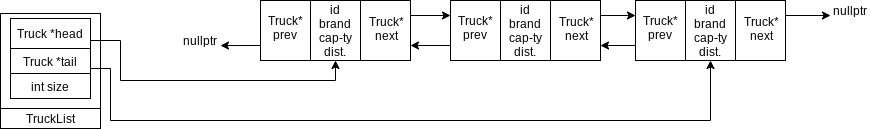
\includegraphics[width=0.9\linewidth]{photo/list_schema}
    \caption{Схема списка}
    \label{list_schema}
\end{figure}

\subsection*{Структуры}

Грузовик Truck представлен в памяти программы в виде структуры с следующими полями:

\begin{itemize}
    \item int id; -- идентификатор грузовика
    \item float capacity; -- максимальна масса груза
    \item int transportation\_distance; -- дальность перевозки
    \item std::string brand; -- марка
    \item Truck *prev; -- указатель на предыдущий элемент
    \item Truck *next; -- указатель  на следующий элемент
\end{itemize}

Структура для работы с элементами списка TruckList сожержит следующие поля:

\begin{itemize}
    \item Truck *head; -- указатель на первый элемент списка
    \item Truck *tail; -- указатель на последний элемент списка
    \item int size; -- количество элементов в списке
\end{itemize}

Структура для высокоуровневой работы со списком TruckDataBase сожержит единственное поле:

\begin{itemize}
    \item TruckList list{}; -- список
\end{itemize}

Для получения команд от пользователя создана структура Cmd с следующими полями:

\begin{itemize}
    \item Command command = Command::NONE; -- команда к выполнению
    \item std::string command\_str{}; -- введённая команда
    \item const std::string prompt = "LR \$>"; -- приглашение командной строки
    \item TruckDataBase *tp; -- указатель на БД, над которой производится выполнение команды
\end{itemize}

Command -- перечисление, содержащее возможные команды.
Состоит из:

\begin{itemize}
    \item Add -- добавить элемент в список
    \item Load -- загрузить список из файла
    \item Save -- сохранить список в файл
    \item Print -- напечатать элемент по индексу
    \item PrintAll -- напечатать все элементы
    \item Help -- справка
    \item Exit -- выход
    \item Skip -- (пустая команда)
    \item NONE -- неопределённая команда
\end{itemize}

Структуры и их взаимосвязи представлены
в виде диаграммы классов на рис.\ref{class_diagram}

\begin{figure}[htp!]
    \centering
    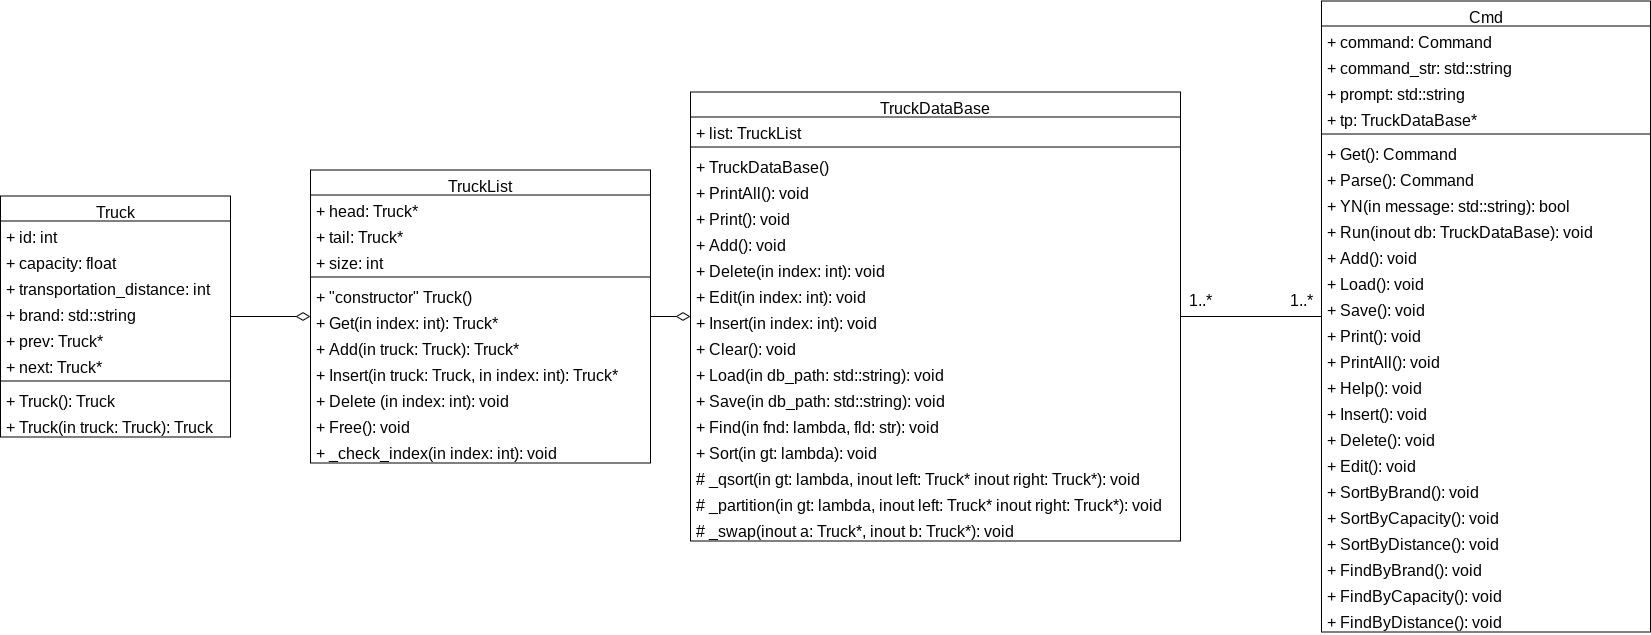
\includegraphics[width=0.9\linewidth]{photo/class_diagram}
    \caption{Диаграмма классов по програмным структурам}
    \label{class_diagram}
\end{figure}